\section{Problem statement and model}
\label{sec:Chapter_III}
\subsection{Problem statement}

An instance consists of $n$ jobs, $N_M$ robotic arms, and $N_A$ vehicles (AGVs), operating on a shop-floor road network represented as a graph.
Job $j$ has a fixed chain of $n_j$ operations $O_{j1}\to\cdots\to O_{jn_j}$; operation $O_{ji}$
may be processed on any robotic arm in its option set $\Omega_{ji}\subseteq M$, taking time
$t^P_{jim}$ on arm $m$, a value that depends on the chosen arm. Robotic arms occupy fixed nodes of the graph, and jobs are moved between these nodes by the fleet.
Solving an instance means determining four groups of decisions at once:

\begin{enumerate}[label=(\roman*),leftmargin=*,topsep=2pt,itemsep=1pt]
\item assign each operation $O_{ji}$ to some robotic arm $m\in\Omega_{ji}$;
\item sequence the operations assigned to each robotic arm;
\item assign the induced transport tasks to vehicles and sequence the tasks of each vehicle;
\item plan a path on the graph for every vehicle move, conflict-free in time and space, with waiting allowed.
\end{enumerate}

The objective is to minimize the makespan $C_{\max}$.

\begin{table}[t]
\caption{Notation.}
\label{tab:notation}
\small
\begin{tabular}{@{}ll@{}}
\toprule
Symbol & Meaning \\
\midrule
$J=\{1,\dots,n\}$, $O_{ji}$ & set of jobs; the $i$-th operation of job $j$, $i\le n_j$ \\
$M=\{1,\dots,N_M\}$, $\Omega_{ji}\subseteq M$ & set of robotic arms; option set of $O_{ji}$ \\
$t^P_{jim}$ & processing time of $O_{ji}$ on arm $m\in\Omega_{ji}$ \\
$K=\{1,\dots,N_A\}$ & homogeneous unit-load vehicles \\
$G=(V,E)$, $\tau_e$ & shop-floor graph; traversal time of corridor $e\in E$ \\
$v_0$, $\mathrm{loc}(m)$ & load/unload point; node occupied by arm $m$ \\
$t^{*}(a,b)$ & shortest-path time from $a$ to $b$ in $G$, ignoring contention \\
$\delta_{\mathrm{ret}}\in\{0,1\}$ & whether a finished job returns to $v_0$ (baseline value $1$) \\
$S_{ji}$, $C_{ji}$, $A_{ji}$ & start, completion, and material-arrival times of $O_{ji}$ \\
$C_{\max}$ & makespan \\
\bottomrule
\end{tabular}
\end{table}

\subsection{Modelling assumptions}
\label{sec:assumptions}

\begin{enumerate}[label=\textbf{A\arabic*.},leftmargin=*,topsep=2pt,itemsep=2pt]
\item \textbf{Static instance and complete information.} All $n$ jobs are already at $v_0$ at time $t=0$; there are no release dates or due dates. Processing data, the layout $G$, and the vehicle states are all known at planning time.

\item \textbf{Jobs.} Each job has a fixed precedence chain. Processing and transport are non-preemptive, jobs cannot be split,
and there are no exogenous precedence constraints among different jobs.

\item \textbf{Robotic arms: partial flexibility and heterogeneous processing times.} Each operation $O_{ji}$ may be processed on any
$m\in\Omega_{ji}$; most operations satisfy $|\Omega_{ji}|\ge 2$, and full flexibility
$\Omega_{ji}=M$ is a special case. Processing times vary with the chosen arm, and the arms need not share a uniform ranking by speed: when
$m\neq m'$, $t^P_{jim}$ and $t^P_{jim'}$ need not be proportional. An arm processes only
one operation at a time and does not fail during the planning horizon; sequence-dependent setup times are folded into $t^P_{jim}$.

\item \textbf{Buffers and loading.} The input and output buffers of each arm, and the storage at $v_0$, have ample capacity,
so blocking does not occur. Loading and unloading times are negligible and do not occupy the arm.

\item \textbf{Vehicles.} The $N_A$ vehicles are homogeneous and unit-load, and travel at constant speed whether empty or loaded; acceleration, deceleration, and
battery charge are not modelled. All vehicles stand empty at $v_0$ at $t=0$ and are immediately available. A transport task is a one-way move---from $v_0$
to the first arm, between two successive distinct arms, or, when $\delta_{\mathrm{ret}}=1$, from the last arm
back to $v_0$; any vehicle may execute any task,
so successive moves of the same job may be relayed across different vehicles. After unloading, a vehicle is not forced back to $v_0$; it
repositions according to its own task chain, and its departure time may be postponed by the routing layer.

\item \textbf{Road network and conflict-freedom.} $G$ is strongly connected, and the traversal time $\tau_e$ of each corridor $e\in E$ is a known constant. Corridors are
\emph{exclusive} resources: the two directions of each corridor $e$ share a single reservation, so at most one vehicle occupies $e$ at any time, which rules out
both head-on conflicts and same-direction overtaking. Occupancy intervals are half-open, $[t,\,t+\tau_e)$, so a second vehicle may enter exactly at
$t+\tau_e$. Nodes have berths of ample capacity, independent of the traversal resources; waits therefore occur at berths
and are always permitted.

\item \textbf{Out of scope.} Machine and vehicle failures, finite buffers and blocking, battery charging, and dynamic
job arrivals~\cite{gui2023dynamic,xiong2024dynamic} are left to future work (item~(5) of Section~\ref{sec:future_work}).
\end{enumerate}

Of these, A1, A2, A4, and A5 are standard assumptions in the FJSP\_PT literature~\cite{xin2025review}. The features that define our problem are A3 (machine-dependent processing times on partially flexible robotic arms) and A6 (contention stated as an explicit exclusive-resource constraint rather than a constant travel-time matrix);
as a result, transport duration is an output of the routing decision, not a fixed input parameter.
Deadlock-freedom is not an assumption: Proposition~\ref{prop:decodable} in Section~\ref{sec:upper} uses A4 and A6 to prove that any assignment and operation sequence can be decoded into a conflict-free, deadlock-free timetable, so the search need not repair infeasible solutions.

\subsection{Decision variables and induced transport tasks}

Let $x_{jim}\in\{0,1\}$ indicate that $O_{ji}$ is assigned to robotic arm $m$; write $\mathrm{m}(j,i)$ for the chosen arm and
$d_{ji}=\mathrm{loc}(\mathrm{m}(j,i))$ for the node of that arm. When $\delta_{\mathrm{ret}}=1$,
a zero-duration \emph{dummy operation} $O_{j,n_j+1}$ at $v_0$ is appended to each job, representing the return to the load/unload point after completion;
in this way return moves and intermediate moves share the same task notation, and the makespan is always the completion time of each job's last operation.

Unlike in a vehicle routing problem, transport tasks are not part of the input; they are \emph{induced} by the assignment:
\begin{equation}
\label{eq:tasks}
\mathcal{T}(x)=\Bigl\{\,(j,i)\ :\ d_{j,i-1}\neq d_{ji}\,\Bigr\},
\qquad d_{j0}\equiv v_0 ,
\end{equation}
where task $(j,i)$ moves job $j$ from $d_{j,i-1}$ to $d_{ji}$ and becomes ready at time
$r_{ji}=C_{j,i-1}$ (with the convention $C_{j0}=0$). If two successive operations are placed on the same arm, no
transport task is created. Thus both the \emph{number} and the \emph{endpoints} of transport tasks are consequences of decision group~(i): an assignment that keeps a job
on the same arm throughout needs only two moves, whereas an assignment that changes arm at every operation needs $n_j+1$ moves.
Assignment of tasks to vehicles is indicated by $y_{tk}\in\{0,1\}$, with
$\sum_{k\in K}y_{tk}=1$ for each $t\in\mathcal{T}(x)$; tasks given to the same vehicle are ordered into a sequence.

In a constant travel-time matrix model, the assignment likewise determines the number of moves and their endpoints, but the duration of each move is a constant in the matrix, and corridor occupancy does not enter the model.
In this paper, the same assignment also determines on which corridors those moves contend with one another.

\subsection{Timing relations and feasibility}

Write $p_{ji}=\sum_{m\in\Omega_{ji}}x_{jim}t^P_{jim}$ for the processing time on the chosen arm. Assignment, precedence, and
the unit capacity of each arm give
\begin{align}
\sum_{m\in\Omega_{ji}} x_{jim} &= 1, & \forall j,i,
\label{eq:assign}\\
C_{ji} &= S_{ji}+p_{ji}, & \forall j,i,
\label{eq:dur}\\
S_{ji} &\ \ge\ A_{ji}, & \forall j,i,
\label{eq:material}\\
S_{j'i'}\ \ge\ C_{ji}\ \ \vee\ \ S_{ji} &\ \ge\ C_{j'i'}
& \forall (j,i)\neq(j',i')\ \text{on the same arm},
\label{eq:disj}
\end{align}
where $A_{ji}$ is the time at which the job actually appears at $d_{ji}$. If $(j,i)\notin\mathcal{T}(x)$, the job is
already there and $A_{ji}=C_{j,i-1}$. Otherwise $A_{ji}$ is produced by the vehicle that carries task $(j,i)$: write
$a^{\mathrm{E}}_{ji}$ for the time at which that vehicle reaches the pickup node after its empty leg; then
\begin{equation}
\label{eq:load}
\ell_{ji}=\max\bigl(a^{\mathrm{E}}_{ji},\ r_{ji}\bigr),
\qquad
A_{ji}=\text{arrival time of the loaded leg departing at } \ell_{ji},
\end{equation}
i.e.\ the vehicle may wait for the job, and the job may wait for the vehicle. Whether empty or loaded, each leg is a walk
$(e_1,\dots,e_q)$ in $G$ whose corridor entry times $\eta_1,\dots,\eta_q$ satisfy
\begin{equation}
\label{eq:walk}
\eta_1 \ \ge\ \sigma, \qquad
\eta_{l+1}\ \ge\ \eta_l+\tau_{e_l}, \quad l=1,\dots,q-1,
\end{equation}
where $\sigma$ is the time at which the leg may start.
If $\eta_{l+1}=\eta_l+\tau_{e_l}$, the vehicle enters the next corridor without stopping; if $\eta_{l+1}>\eta_l+\tau_{e_l}$, the difference is the vehicle's waiting time at a berth. The leg ends at $\eta_q+\tau_{e_q}$.
Finally, the corridor-contention constraint is
\begin{equation}
\label{eq:excl}
\bigl[\eta,\ \eta+\tau_e\bigr)\ \cap\
\bigl[\eta',\ \eta'+\tau_e\bigr)\ =\ \emptyset
\end{equation}
This constraint holds for any two distinct occupancies of the same corridor $e$, regardless of direction and of which vehicles are involved; it is also the only constraint in the model that couples different jobs through \emph{space} rather than through a shared arm. The objective is
\begin{equation}
\label{eq:obj}
\min\ C_{\max},\qquad
C_{\max}=\max_{j\in J}\ C_{j,\,n_j+\delta_{\mathrm{ret}}} .
\end{equation}

In a semi-active schedule (every operation starts at the earliest time the constraints allow), Eqs.~\eqref{eq:material} and \eqref{eq:disj} tighten to
\begin{equation}
\label{eq:bind}
S_{ji}=\max\bigl(A_{ji},\ F_{\mathrm{m}(j,i)}\bigr),
\end{equation}
where $F_m$ is the completion time of the operation sequenced immediately before $O_{ji}$ on arm $m$; that is, the start time is the later of the job's arrival and the completion of the preceding operation on that arm. Section~\ref{sec:Chapter_IV} uses this to attribute a postponed start to waiting for the workpiece or waiting for the arm.

\subsection{Relation to FJSP\_PT}
\label{sec:fjsppt}

Once Eq.~\eqref{eq:excl} is removed, legs no longer occupy corridors against one another, so every leg can take a shortest path without waiting along the way. Transport durations collapse to the constant matrix $t^{*}(a,b)$,
and the model becomes flexible job shop scheduling with transportation (FJSP\_PT). The two problems therefore differ only in this set of corridor-exclusivity constraints: with them, the duration of a move is jointly determined by the vehicles' paths; without them, the duration is an input parameter.
The resulting $t^{*}$ is used later as a lower bound, and in the open-loop baseline to estimate arrival times by unimpeded travel time.

Relative to work that likewise supplies an explicit road network, the difference lies in what is reserved. van Os and Basten~\cite{vanos2026exact}
reserve \emph{nodes}: two vehicles may not occupy the same node at the same time, nor swap nodes. This paper reserves \emph{edges}: corridors are exclusive in both directions, and at most one vehicle occupies a corridor at any time.
Lyu et al.~\cite{lyu2019approach} likewise make corridors exclusive in both directions, but additionally allow each node to hold only one vehicle at a time; this paper instead provides berths of ample capacity at nodes for vehicles to wait in, consistent with how Assumption A4 treats arm buffers and the storage at $v_0$ and corresponding to the vehicle standby areas beside workstations in real shops, so congestion occurs only on corridors.
The reasons why the instances cannot be compared directly are given under limitation~(1) in Section~\ref{sec:limitations}.

\subsection{Computational complexity}

\begin{prop}
\label{prop:np_hard}
The problem defined by Eqs.~\eqref{eq:assign}--\eqref{eq:obj} is strongly NP-hard, and it remains so when every operation satisfies
$\Omega_{ji}=M$.
\end{prop}

\begin{proof}
Restrict to instances in which $\tau_e=0$ for every $e\in E$, each robotic arm is connected to $v_0$ by a dedicated corridor,
and $N_A=n$. Every leg then takes zero time and occupies the empty half-open interval $[t,t)=\emptyset$, so Eq.~\eqref{eq:excl}
holds trivially and no vehicle can delay another; moreover, because each job has a vehicle of its own, Eq.~\eqref{eq:load} never binds and
$A_{ji}=C_{j,i-1}$. What remains is exactly
Eqs.~\eqref{eq:assign}--\eqref{eq:disj} with $A_{ji}=C_{j,i-1}$, i.e.\ the flexible job shop scheduling problem with unrelated machines. Two of its
special cases are already strongly NP-hard: taking $|\Omega_{ji}|=1$ everywhere reduces it to the classical job shop problem, which is
strongly NP-hard already with three machines; taking $\Omega_{ji}=M$ and $n_j=1$ reduces it to makespan minimization on unrelated parallel
machines, which contains identical-parallel-machine scheduling and is strongly NP-hard when the number of machines is part of the input.
Flexible job shop scheduling in general is itself strongly NP-hard~\cite{dauzereperes2024fjsp}. Each of the restrictions above is a
polynomial reduction, so the general problem is strongly NP-hard; the second special case also shows that full flexibility does not make the problem easier.
\end{proof}

The reduction in Proposition~\ref{prop:np_hard} sets corridor traversal times to zero and thereby excludes vehicle contention. This shows that the problem is already strongly NP-hard even without corridor contention.
If decisions~(i)--(iii) are then fixed, the remaining path planning is still a conflict-free multi-agent routing problem~\cite{gao2023mapf}, in which the release times and endpoints of the tasks are determined by the operation chains and the assignment and constrain one another.
Conflict-free routing therefore adds constraints on top of the scheduling difficulty rather than replacing it. Exact methods already exist at small scale: van Os and Basten~\cite{vanos2026exact} use logic-based Benders decomposition
to solve most benchmark instances under the same problem setting to proven optimality. This paper targets sizes beyond the practical reach of that exact decomposition.

\subsection{Instance features}
\label{sec:features}

This paper holds instance size fixed and varies only structure; the effect of size itself is discussed under limitation~(1) in Section~\ref{sec:limitations}.
Each instance records the following features. The first four are quantities common in the scheduling literature; Xin et al.~\cite{xin2025review} note that $\bar{T}_t/\bar{T}_p$ among them is likely to affect algorithm performance.


\begin{itemize}[leftmargin=*,topsep=2pt,itemsep=1pt]
  \item $\bar{T}_t/\bar{T}_p$: the mean shortest-path travel time between arm nodes divided by the mean processing time, i.e.\ the ratio of transport time to processing time.
  \item Heterogeneity $H$: the coefficient of variation of each operation's processing times over its optional arms, averaged over all operations (operations with $|\Omega_{ji}|=1$ contribute $0$).
  $H=0$ means that the optional arms have identical processing times: reassignment does not affect processing time but can still be used to avoid congestion.
  As $H$ grows, processing-time differences increasingly dominate the assignment and the room for reassignment to avoid congestion shrinks accordingly, so we do not expect the gain to rise with $H$; the measurements grouped by $H$ in Section~\ref{sec:whichcongestion} agree with this.
  \item Flexibility $F=\operatorname{mean}_{ji}|\Omega_{ji}|/N_M$: the mean number of optional arms per operation as a fraction of all arms, i.e.\ the scope of reassignment.
  \item $N_A/N_M$: the vehicle-to-arm ratio. A smaller ratio makes the bottleneck more likely to lie in transport; a larger ratio, in processing.
\end{itemize}

We also record two quantities that are meaningful only on an explicit road network, describing the severity of congestion and the part of it that reassignment can avoid.
Let $\mathrm{cut}(v_0)$ be a smallest set of corridors whose removal disconnects the load/unload point $v_0$ from every robotic arm.

\begin{itemize}[leftmargin=*,topsep=2pt,itemsep=1pt]
  \item Contention intensity: on the initial random population, the share of total travel time that is yielding wait. It is determined by the instance structure rather than supplied as an input parameter; we use it to order the instances, and the per-instance values are given in Table~\ref{tab:instances}.
  \item $|\mathrm{cut}(v_0)|$ (funnel width): an upper bound on the number of vehicles that can leave the load/unload point at the same time. The value $1$ means that every vehicle must pass through the same corridor to leave. The layout family (Family~A) varies contention by adding or removing such parallel exits; relative to \texttt{high}, \texttt{funnel} halves this value.
\end{itemize}

Each instance carries a composite lower bound
$\mathrm{LB}=\max(\mathrm{LB}_{\text{chain}},\mathrm{LB}_{\text{load}},
\mathrm{LB}_{\text{cut}})$, computed directly from the instance data. The three components each relax a different part of the model, and none is always the largest on every instance.
$\mathrm{LB}_{\text{chain}}$ takes, for each job, ``the shortest inbound trip $+$
$\sum_i \min_{m\in\Omega_{ji}}t^P_{jim}$ $+$ the shortest return trip'', i.e.\ it ignores inter-arm moves and all queueing.
$\mathrm{LB}_{\text{load}}$ takes $\sum_{j,i}\min_m t^P_{jim}/N_M$, i.e.\ it ignores operation precedence and transport.
$\mathrm{LB}_{\text{cut}}$ exploits the funnel: when $\delta_{\mathrm{ret}}=1$ each job crosses
$\mathrm{cut}(v_0)$ twice; spreading the $X=2n$ crossings over the corridors of that cut so as to minimize the load on the busiest one yields
\begin{equation}
\label{eq:lbcut}
C_{\max}\ \ge\ X\Bigl/\sum_{e\in \mathrm{cut}(v_0)}\tau_e^{-1}.
\end{equation}
On the instances of this paper, the largest of the three is $\mathrm{LB}_{\text{cut}}$ (on eight of the ten instances) or
$\mathrm{LB}_{\text{chain}}$ (on the other two), and $\mathrm{LB}_{\text{load}}$ is never the largest---which agrees with an instance design that concentrates contention at the load/unload exit.
The bound is fairly loose: its gap to the best known solution is roughly between \LBGapLo{} and \LBGapHi{}, so it is used only to check the order of magnitude, not to prove that a solution is near-optimal.

\section{Closed-loop bilevel framework}
\label{sec:Chapter_IV}
\subsection{Overview: routing-in-the-loop evaluation and the decision path}
\label{sec:overview}

The framework assigns the four groups of decisions of Section~\ref{sec:Chapter_III} to two levels. The input is an instance: the operation chains of the jobs,
the option sets and processing times of the arms, the fleet size, and the corridor network. The upper level searches over assignment and sequencing with a memetic algorithm~\cite{zhang2024memetic}; in the middle,
an event-driven decoder translates one upper-level candidate into a sequence of precedence-constrained transport tasks; the lower level turns
this sequence into conflict-free paths by time-window reservation.
The output is an executable conflict-free timetable and its makespan.
Relative to two-stage schemes or schemes that correct only once, the difference lies not in having two levels but in how the routing result enters the schedule: the content and direction of the feedback, and whether every candidate receives it.


\begin{description}[leftmargin=0pt,topsep=3pt,itemsep=3pt]
  \item[The evaluation path, i.e.\ \emph{routing-in-the-loop evaluation}.]
  In every generation, the fitness of each candidate is the makespan after the lower level has completed conflict-free routing of all transport tasks, yielding wait included.
  The upper level takes this value as its objective, rather than the makespan computed on the assumption that vehicles never interfere and always travel unimpeded.
  \item[The decision path.]
  Vehicle selection reads the current reservation table, instead of learning the outcome only after the paths have been generated.
  The mechanism is \emph{reservation-table-aware dispatching}: for each candidate vehicle, the earliest feasible times of the empty leg and then the loaded leg are obtained by a trial query on the reservation table (the trial query does not write the final timetable), and the vehicle with the earliest feasible delivery is selected, rather than the vehicle whose arrival is earliest by the unimpeded-shortest-path estimate.
\end{description}

The contributions of the two paths to makespan are measured separately in Section~\ref{sec:Chapter_V}.
The two further inter-layer interfaces implemented are an extra cost on occupied corridor--time slots (hereafter, surcharge) and reassignment or resequencing from the yield record; their constructions are given in Sections~\ref{sec:interface} and~\ref{sec:ls}, and the control results in Section~\ref{sec:Chapter_V}.

The structure of the framework is shown in Figure~\ref{fig:framework}. The two paths enter the upper level at different places, and the computational cost of a single evaluation therefore differs as well.

%% 本图由 fig/fig_framework_CN.py 生成,是一张示意图,不含任何数据。
%% 注意不要复用 fig/fig_hdp_architecture*.pdf,那是上一篇论文的 HDP 框架。
\begin{figure*}[t]
\centering
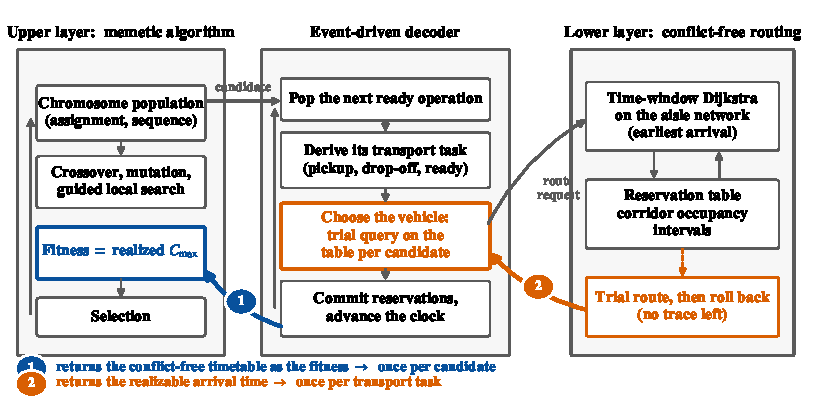
\includegraphics[width=\textwidth]{fig/fig_framework.pdf}
\caption{The closed-loop bilevel framework. The upper level searches over assignment and sequencing with a memetic algorithm, the lower level performs conflict-free routing by time-window reservation,
and an event-driven decoder in the middle translates one upper-level candidate into a sequence of transport tasks.
The two feedback paths are distinguished by colour and enter the upper level at different places:
path~1 (blue, marked 1) returns the conflict-free timetable completed by the lower level as fitness, once per candidate;
path~2 (orange, marked 2) runs a trial query on the reservation table for the earliest feasible delivery time of the two legs before a vehicle is chosen, once per transport task; the trial query does not write the final timetable.
The four-level baseline ladder of Section~\ref{sec:Chapter_V} is arranged by whether these two paths are open.}
\Description{Schematic of the closed-loop bilevel framework: an upper memetic
search layer, an event-driven decoder, and a lower time-window reservation
routing layer, with two colour-coded feedback paths entering the upper layer at
different places---the evaluation path returning a realized makespan once per
candidate, and the decision path returning a realizable arrival time once per
transport task.}
\label{fig:framework}
\end{figure*}

\subsection{Lower level: time-window reservation and conflict-free routing}
\label{sec:router}

\subsubsection{Reservation table}
The only contended resource is the corridor (assumption~A6), so the reservation table maps each corridor to a time-ordered list of half-open occupancy intervals $[t,\,t+\tau_e)$, each labelled with the vehicle and task that occupy it.
The table supports four operations: query the earliest feasible entry time no earlier than a given instant; write an occupancy; revoke every occupancy of a given task; and save the current table state and restore it after a trial query (checkpoint and rollback).
Nodes are not reserved: traversing a node takes zero time, and waits occur at berths (assumption~A6 already separates berths from the traversal resource).
Only one resource, the corridor, therefore needs to be reserved, and both the lower-level conflict-free path planner (hereafter, the router) and a checker independent of the decoder inspect only corridor occupancy.

\subsubsection{Time-window Dijkstra}
A leg is planned by a label-setting search. A label $(u,t)$ means ``standing at the berth of node $u$ at time $t$'', and its cost is $t$ (Algorithm~\ref{alg:route}).
When a corridor leaving the current node is examined, the reservation table is queried for the earliest feasible entry time $t'\ge t$; the gap $t'-t$ is the time the vehicle waits at the berth of $u$.
The wait in Eq.~\eqref{eq:walk} is therefore produced directly by the search and need not be modelled separately.
Within one decoding, paths already written to the reservation table are not revoked, so vehicles are planned one after another in the fixed order in which the decoder generates tasks, and a later-planned vehicle yields to an earlier-planned one.

\begin{lem}[One earliest-arrival label per node suffices]
\label{lem:label}
Keeping only the earliest-arrival label at each node is sufficient to obtain a path that reaches the destination earliest under the current reservation table.
\end{lem}

\begin{proof}
  Berths have ample capacity and do not occupy the traversal resource (A6), so a vehicle that has stood at $u$ since time $t$ need only wait further until $t'$
  in order to take any continuation that a vehicle arriving at $u$ only at $t'>t$ could take.
  An earlier-arrival label is therefore never worse.
  Moreover, the later the query time to the reservation table, the fewer (never more) the still-feasible entry slots,
  so the time to enter corridor $e$ and finish traversing it,
  $t\mapsto R.\textsc{EarliestEntry}(e,t,\tau_e)+\tau_e$,
  is non-decreasing in $t$.
  The search extracts labels in increasing order of arrival time, and the first time the destination is extracted is the earliest arrival.
\end{proof}

Ordinary Dijkstra therefore suffices, and there is no need for the per-interval labelling of Safe Interval Path Planning (SIPP)~\cite{kasaura2022sipp}; if a second criterion is introduced (for example, a surcharge on corridor--time slots), earlier arrival is no longer always better, and a multi-label search is required (Section~\ref{sec:interface}).

\begin{algorithm}[t]
  \caption{\textsc{Route}: conflict-free planning of a single leg}
  \label{alg:route}
  \small
  \begin{algorithmic}[1]
  \Require origin $s$, destination $g$, earliest departure time $t_0$, reservation table $R$, write-to-table flag \textit{commit}
  \Ensure a sequence of arrival time and corridor occupancy intervals; if \textit{commit} is true, those intervals are also written to $R$
  \State place the label $(s,t_0)$ in a priority queue keyed by (time, node id)
         \Comment{ties in time broken by node id, so the order is deterministic}
  \While{the queue is nonempty}
    \State extract the label $(u,t)$ of least key
    \If{$u=g$} \State backtrack to obtain the occupancy intervals; if \textit{commit} is true, write them to $R$ one by one;
         \Return arrival time $t$ \EndIf
    \ForAll{corridors $e=(u,v)$ leaving $u$}
      \State $t_{\text{in}} \gets R.\textsc{EarliestEntry}(e,t,\tau_e)$
         \Comment{wait at the berth of $u$ until $t_{\text{in}}$}
      \State if $t_{\text{in}}+\tau_e$ is strictly earlier than the incumbent arrival at $v$, update the label $(v,\ t_{\text{in}}+\tau_e)$
    \EndFor
  \EndWhile
  \State \Return failure \Comment{should not occur when $G$ is strongly connected; see the text}
  \end{algorithmic}
\end{algorithm}

The number of reservations is finite, time is bounded, and $G$ is strongly connected, so a path always exists: in the worst case the vehicle waits until every existing occupancy has ended and then travels along an unimpeded shortest path.
This guarantees that Proposition~\ref{prop:decodable} below holds, so the search need not repair infeasible solutions.
A single call costs $O\bigl(|E|\,(W^{2}+\log|V|)\bigr)$: at most $|E|$ corridors are examined; for each, $O(W)$ candidate entry times are enumerated, each candidate is tested for overlap in $O(W)$ time,
and one heap operation of $O(\log|V|)$ is performed, where $W$ is the mean number of reserved intervals per corridor.
If the reservation table were replaced by an ordered structure supporting a logarithmic-time earliest-entry query, the complexity would drop to $O\bigl(|E|(\log W+\log|V|)\bigr)$; the implementation in this paper uses the linear scan above.

Running the same search on an empty reservation table over all pickup--delivery node pairs yields the unimpeded shortest-path matrix $t^{*}$ of Section~\ref{sec:Chapter_III}.
It is used in three places: estimating arrival times by unimpeded time in open-loop configurations, the proximity term in the reassignment neighbourhood, and the transport times of the two-stage baseline; it is also the admissible lower bound used by the pruning of Section~\ref{sec:speedup}.


\subsection{Upper level: encoding and event-driven decoding}
\label{sec:upper}

\subsubsection{Chromosome encoding}
Let the total number of operations be $N$. An individual consists of two segments: a \emph{machine-assignment vector} of length $N$, indexed by a fixed enumeration, whose $k$-th component is the robotic arm chosen for the $k$-th operation from $\Omega_{ji}$;
and an \emph{operation sequence}, a permutation that allows a job to appear more than once---job $j$ appears $n_j$ times, and its $x$-th appearance stands for $O_{jx}$.
The sequence supplies a global order: the relative order of operations that share a robotic arm is read from it.

When $\delta_{\mathrm{ret}}=1$, each job appears once more in the sequence, corresponding to the dummy operation of Section~\ref{sec:Chapter_III} (location fixed at $v_0$, processing time zero).
Return transport therefore uses the same assignment and sequencing as intermediate transport, and the decoder needs no separate branch.

Which vehicle a task is given to is not written into the chromosome; it is decided at decode time (Section~\ref{sec:dispatch}).
A third segment for dispatching would enlarge the search space and would no longer guarantee that every chromosome is decodable, so a repair operator would be required.


\subsubsection{Event-driven decoder}
The decoder (Algorithm~\ref{alg:decode}) implements the evaluation path. It sweeps the operation sequence from left to right, maintaining the idle
time of each robotic arm, the current node and ready time of each job, and the current node and available time of each vehicle. When the
arm of an operation differs from the job's current location, a transport task of Eq.~\eqref{eq:tasks} is generated, a vehicle is chosen, and two paths are planned against the \emph{live}
reservation table: an empty leg to the pickup point and a loaded leg to the destination, joined by Eq.~\eqref{eq:load}.
The operation then starts by Eq.~\eqref{eq:bind}; the decoder also records what determined the start---the arrival of the job (waiting for the workpiece) or the completion of the previous operation on that arm (waiting for the arm)---and later tracing of a postponed start takes this record as authoritative.

\begin{algorithm}[t]
\caption{\textsc{Decode}: fitness from a complete conflict-free simulation}
\label{alg:decode}
\small
\begin{algorithmic}[1]
\Require instance, road network, assignment $x$, operation sequence
\Ensure makespan, timetable, per-corridor yield statistics
\State for every robotic arm set $F_m\gets 0$; for every job set $\mathrm{pos}_j\gets v_0$,
       $\mathrm{ready}_j\gets 0$
\State for every vehicle set $\mathrm{loc}_k\gets v_0$, $\mathrm{avail}_k\gets 0$; clear the reservation table
\ForAll{operations $O_{ji}$ taken in sequence order (dummy operations included)}
  \State $m\gets$ the robotic arm of $O_{ji}$ under $x$; $d\gets \mathrm{loc}(m)$
  \If{$\mathrm{pos}_j=d$}
     \State $A_{ji}\gets \mathrm{ready}_j$ \Comment{successive operations on the same arm; no transport task}
  \Else
     \State choose vehicle $k$ (Section~\ref{sec:dispatch})
     \State $a^{\mathrm{E}}\gets\textsc{Route}(\mathrm{loc}_k,\mathrm{pos}_j,
            \mathrm{avail}_k,R,\text{true})$;\ \ $\ell\gets\max(a^{\mathrm{E}},
            \mathrm{ready}_j)$ \Comment{the empty leg occupies corridors as well}
     \State $A_{ji}\gets\textsc{Route}(\mathrm{pos}_j,d,\ell,R,\text{true})$;\ \
            $\mathrm{loc}_k\gets d$;\ \ $\mathrm{avail}_k\gets A_{ji}$
     \State accumulate yielding time by corridor
  \EndIf
  \State if $F_m>A_{ji}$ then $\texttt{bind}\gets\texttt{machine}$, else
         $\texttt{bind}\gets\texttt{arrive}$ \Comment{record waiting for the arm or waiting for the workpiece}
  \State $S_{ji}\gets\max(A_{ji},F_m)$;\ \ $C_{ji}\gets S_{ji}+p_{ji}$;\ \
         $F_m\gets C_{ji}$;\ \ $\mathrm{pos}_j\gets d$;\ \
         $\mathrm{ready}_j\gets C_{ji}$
\EndFor
\State \Return $C_{\max}=\max_{j,i} C_{ji}$, the timetable, and the per-corridor yield statistics
\end{algorithmic}
\end{algorithm}

Decoding is deterministic: reservations are written in the order in which the decoder generates tasks, and ties in time are broken by a fixed rule at both sites---the routing label queue is keyed by (arrival time, node id) and a label is updated only when the new arrival is strictly earlier;
dispatching scans vehicles in increasing id order and keeps the first strictly better one (Section~\ref{sec:speedup}).
A chromosome therefore always corresponds to a unique timetable, and evaluation is deterministic. The seed-paired, equal-budget comparisons of Section~\ref{sec:Chapter_V} depend on this.

\begin{prop}[Every chromosome is decodable]
  \label{prop:decodable}
  For any machine assignment and any operation sequence, Algorithm~\ref{alg:decode} terminates and returns a conflict-free, deadlock-free timetable of finite makespan. The search therefore need not invoke a repair operator.
\end{prop}

\begin{proof}
  By the encoding, the operation sequence is a topological order of each job's precedence constraints: the $x$-th appearance of a job stands for its $x$-th operation, so $\mathrm{ready}_j$ is already known when it is read.
  Ample buffers (A4) mean that an operation is never blocked for lack of storage, so once the job has arrived, Eq.~\eqref{eq:bind} always supplies a finite start time.
  Each \textsc{Route} call returns in finite time by the argument following Algorithm~\ref{alg:route}, and occupies only slots that are still free on the reservation table, so Eq.~\eqref{eq:excl} holds by construction.
  Deadlock-freedom likewise holds by construction: the corridor is the only contended resource (A6); waits occur only at berths of ample capacity and do not occupy corridors; every occupancy written to the reservation table ends at a finite time, so there is no circular wait among vehicles; in the worst case a vehicle waits until every existing occupancy has ended and then proceeds.
  The sweep executes $N+n\delta_{\mathrm{ret}}$ times, and each time schedules a finite number of events at finite times.
\end{proof}

%% 原为 4.3 的一个子小节 "Dispatching",现提升为独立一节:它是本文承重的机制,
%% 不应埋在"上层编解码"之下。原 4.4 "What should cross the interface?" 的三种接口
%% 讨论降为本节的一个子小节,作为选定该机制的论证。
\subsection{Reservation-table-aware dispatching}
\label{sec:dispatch}

A vehicle may be chosen either by an unimpeded-shortest-path estimate or by a trial query on the reservation table. The open-loop rule scores each vehicle by
\begin{equation}
\label{eq:rule}
\mathrm{score}(k)=\max\bigl(\mathrm{avail}_k+t^{*}(\mathrm{loc}_k,\text{pickup}),\,
\mathrm{ready}_j\bigr)+t^{*}(\text{pickup},\text{destination}),
\end{equation}
which does not consult the reservation table and may therefore select a vehicle that is geometrically near but whose corridors are already occupied.
The formula is the same as the idle-first dispatching of Li et al.~\cite{li2026framework}, and is also a typical single-attribute rule in surveys of multi-AGV dispatching~\cite{lu2022agv}.

The closed-loop default instead uses \emph{reservation-table-aware dispatching}. For each candidate vehicle, the empty leg is planned and temporarily written to the reservation table, the loaded leg is then planned, the earliest feasible delivery time from this trial query is recorded, and the reservation table is rolled back to its state before the trial query.
The empty leg must be written temporarily first; otherwise the loaded leg cannot see that occupancy, the two legs may be placed in the same time slot on the same corridor, and the trial result would be too early.
The vehicle selected is the one with the earliest feasible delivery, not the one that is best by the unimpeded estimate of Eq.~\eqref{eq:rule}.

Vehicles have identical capability (assumption~A5) and differ only in current location and corridor occupancy, so contention on the reservation table can directly determine which vehicle is selected.

The cost of the mechanism is that the trial query raises the routing calls per transport task from $2$ to at most $2N_A$, so a single evaluation costs about \CostMultBefore{} times as much as under rule-based dispatching.
Unless this overhead is reduced, the makespan gain of the mechanism is offset by the extra computation under an equal wall-clock budget.
The two speed-ups are given in Section~\ref{sec:speedup}; Section~\ref{sec:Chapter_V} therefore compares the two dispatching rules only under the same wall-clock limit.

\subsection{Low overhead: admissible lower-bound pruning and winner-path reuse}
\label{sec:speedup}

Under an equal wall-clock budget, reservation-table-aware dispatching faces the following problem. At an equal number of \emph{generations}, reservation-table-aware dispatching outperforms rule-based dispatching by \GainProbeSameGen{} (Figure~\ref{fig:protocols});
but a single evaluation costs \CostMultBefore{} times as much, so at equal \emph{wall-clock time} this gain is offset by the extra computational overhead and the net effect is close to zero.
Hence, as long as the cost multiple can be reduced without changing any selection, the gain of the mechanism becomes visible. This subsection gives two such speed-ups, both of which \emph{provably do not change the selected vehicle or the timetable}.

\paragraph{Admissible lower-bound pruning.}
Conflict-free routing can only be \emph{later} because of yielding; it can never be faster than the shortest path that ignores contention. The estimate of Eq.~\eqref{eq:rule} used by the open-loop rule is therefore an \emph{admissible lower bound} on the realized delivery time:
\begin{equation}
\label{eq:lb_dispatch}
\mathrm{lb}(k)=\max\bigl(\mathrm{avail}_k+t^{*}(\mathrm{loc}_k,\text{pickup}),\,
\mathrm{ready}_j\bigr)+t^{*}(\text{pickup},\text{destination})\ \le\ \mathrm{est}(k),
\end{equation}
where $\mathrm{est}(k)$ is the earliest feasible delivery time obtained by a complete two-leg trial query for vehicle $k$.
Hence, if a vehicle's lower bound is already no earlier than the current best trial-query delivery time, routing need not be called for it.

\paragraph{Winner-path reuse.}
After the trial query the reservation table is rolled back as a whole, and the winner's two legs are discarded with it; the decoder then replans the winner on the same (restored) reservation table and writes the legs, causing two redundant routing calls.
Since the search is deterministic, the replanned paths are exactly the same as those found in the trial query, so the paths computed for the winner during the trial query can be cached and written directly to the reservation table without recomputation.

\begin{prop}[The two speed-ups do not change the selected vehicle or the timetable]
  \label{prop:speedup_equiv}
  In the implementation, vehicles are queried in increasing id order, and the selected vehicle is replaced only when some vehicle's feasible delivery is strictly earlier than the current best.
  Under this rule, after the pruning of Eq.~\eqref{eq:lb_dispatch} and winner-path reuse are added, the selected vehicle, the occupancies written to the reservation table, and the final timetable are the same as when a complete two-leg trial query is run for every vehicle.
\end{prop}

\begin{proof}
  Consider pruning first. When vehicle $k$ is reached, let the current best trial-query delivery be $\mathrm{est}^{\ast}$.
  If $\mathrm{lb}(k)\ge \mathrm{est}^{\ast}$, then Eq.~\eqref{eq:lb_dispatch} gives
  $\mathrm{est}(k)\ge\mathrm{lb}(k)\ge\mathrm{est}^{\ast}$,
  so $k$'s feasible delivery cannot be strictly earlier, and $k$ would not be selected even if every vehicle received a complete trial query; not calling routing for it leaves the selected vehicle unchanged.
  The reservation table is saved before each trial query and restored afterwards; vehicles for which routing is not called do not rewrite the table and therefore do not affect later queries.
  Consider reuse next: the two legs of the selected vehicle were computed against one and the same reservation-table state, and the restored table is in the same state that the decoder faces when it subsequently writes.
  Since routing is deterministic, replanning in the same state yields the same paths as the cached ones, so writing the cached paths and replanning before writing produce identical occupancy intervals.
\end{proof}

Together the two speed-ups give a \SpeedupProbe{}-fold speed-up, cut routing calls by \RouteCallCut{}, and reduce the cost multiple of a single evaluation from \CostMultBefore{} to \CostMultAfter{}.
These three numbers are the \emph{joint} effect of the two speed-ups: in the experiments they are measured as one on/off switch (Table~\ref{tab:prune}), and are not attributed separately to pruning or reuse.

The effect of pruning varies with fleet size. The tighter the bound and the earlier a good trial-query delivery time is found, the more vehicles need no routing call; the larger the fleet, the more candidates there are, and the total trial-query cost grows approximately linearly with $N_A$.
Measurements in Section~\ref{sec:Chapter_V} show that the pruning effect weakens as the fleet grows, but still cuts \RouteCallCutLo{} of the routing calls on the largest fleet tested.
Taken together, these effects mean that the gain of the mechanism may vanish beyond some fleet size; Section~\ref{sec:whichcongestion} explains that the present number of seeds is not sufficient to determine that size.

\subsection{Two further inter-layer interfaces: surcharges and yield records}
\label{sec:interface}

What the evaluation path and the dispatching trial query read from the lower level are both \emph{realized durations}, i.e.\ traversal times after conflict-free routing. They rank every candidate by its makespan with its own yielding wait included; methods that schedule first and route once obtain a realized duration only once, after the assignment has been fixed. Realized durations, however, do not indicate which decision caused the wait. We therefore implement two further interfaces that carry richer information and compare them against it under an equal wall-clock budget; the results are in Section~\ref{sec:pricing}.

\paragraph{Return an extra cost on corridor--time slots.}
By analogy with the use of shadow prices to coordinate resources in Lagrangian relaxation and column generation, a surcharge can be attached to the contended resource: each corridor--time slot receives a surcharge $\pi(e,b)$, the amount that a vehicle occupying corridor $e$ in time slot $b$ must count in addition to its arrival time,
so that path planning minimizes ``arrival time $+\theta\cdot$ the sum of surcharges of the slots traversed'' (the surcharge coefficient $\theta\ge0$ is the only tunable parameter), and reassignment must likewise pay the surcharge for the traversal it requires.
We implement two estimates: perturbing the capacity of a single slot and re-solving, and a low-cost approximation refreshed each generation.

Mechanistically, a surcharge provides no new information. The wait caused by contention already enters the vehicle's arrival time, then enters the makespan through Eq.~\eqref{eq:bind}, and is counted by the fitness;
attaching a further cost to the same occupancy counts the same delay twice. Later tasks not yet planned may be blocked by reservations written earlier, but that effect is likewise already reflected in the makespan after a complete decode.
Hence, as long as the fitness is taken from a complete conflict-free decode, attaching a congestion cost to the lower-level objective adds no information. We verify this inference only on this one interface.

The main overhead of a surcharge follows from Lemma~\ref{lem:label}: once the surcharge is a second criterion, earlier arrival is no longer always better, and single-label Dijkstra must be replaced by a multi-label Pareto search,
so the cost of a single evaluation rises whether or not the surcharge is non-zero.


\paragraph{Return the yield record.}
The other choice is to return structure. When a yield occurs, path planning already knows the corridor, the time slot, and the transport that first occupied that corridor; the decoder keeps these yield events, not only the total wait.
A record is a triple (corridor, time slot, preceding occupying transport), used to decide which operations local search should change.
It does not enter any objective: the lower level still minimizes arrival time, the upper level still minimizes makespan; only the way the neighbourhood is generated changes.
There is therefore no double-counting of delay. The operators are given in Section~\ref{sec:ls}.

\subsection{Yield-record-guided local search}
\label{sec:ls}
This subsection writes the yield record of the previous subsection as local-search operators, applied to the top-ranked individuals in each generation; all four configurations of the main batch enable it with the same setting. Its critical-chain tracing is also used for the reading of the case study in Section~\ref{sec:casestudy}.

\paragraph{Critical-chain tracing.}
Backtracking from the event that determines the makespan yields a chain. A chain that contains only operations cannot explain why a start was postponed: when the start is waiting for the workpiece, the postponement may come from an unfinished upstream operation, no vehicle being available, or corridor contention, and the three call for different changes.
The backtrack therefore includes transport legs as well, and labels every link with a type (Table~\ref{tab:attrib}): a yield on a loaded leg is recorded as corridor occupancy; an empty leg is classified as ``vehicle'' or ``corridor'' by the share of yielding time in that leg's duration, with threshold $0.5$.
Only the corridor-occupancy class gives a concrete corridor, time slot, and preceding occupying transport, and this is exactly the information that local search uses.

\begin{table}[t]
  \caption{Labels of the links on the critical chain, and the changes that can be taken.
  Only the corridor-occupancy class carries a concrete corridor and time slot, and only it can name the transport that first occupied that corridor.}
\label{tab:attrib}
\footnotesize
\begin{tabular}{@{}llp{2.55cm}@{}}
\toprule
Label & Criterion & Remedy \\
\midrule
\texttt{operation} & a real operation is occupying its robotic arm & --- \\
\texttt{machine} & waiting for the arm: blocked by the preceding operation on that arm
  & resequence \\
\texttt{upstream} & the vehicle arrived first, the material is not yet ready & recurse to $O_{j,i-1}$ \\
\texttt{vehicle} & the material is ready, the vehicle is late, and yielding is a small share of the delay & change vehicle \\
\texttt{corridor} & a yield occurs on a specified corridor in a specified time slot & reassignment or staggering \\
\bottomrule
\end{tabular}
\end{table}

\paragraph{Two families of operators and the acceptance rule.}
\emph{Reassignment: change the processing location.} For at most $L=5$ real operations $O_{ji}$ on the critical chain (with current assignment on robotic arm $m$), each alternative robotic arm
$m'\in\Omega_{ji}\setminus\{m\}$ is scored by
\begin{equation}
\label{eq:reassign}
\mathrm{score}(m')=t^{*}\bigl(d_{j,i-1},\mathrm{loc}(m')\bigr)
+t^{P}_{jim'},
\end{equation}
i.e.\ the sum of the unimpeded travel time from the node $d_{j,i-1}$ of the previous operation to $m'$ and the processing time on $m'$; the lowest-scoring arm produces a neighbour that changes only that one assignment. This allows a longer processing time to be traded for a shorter path with better traffic conditions, which is the reassignment trade-off of this paper.
The score contains no cumulative-yield term, because that term is a total over the whole fleet and the whole planning horizon and is not commensurable with the scale of a single operation.

\emph{Staggering: change the order.} Take the longest corridor-occupancy link on the chain and generate two directed neighbours: advance the blocked operation in the sequence, or postpone the preceding occupying operation, so that the two occupancies no longer overlap.
A move only swaps adjacent appearances of different jobs, leaving the internal order of each job unchanged, so by Proposition~\ref{prop:decodable} the result remains decodable.

The neighbourhood therefore has at most $L+2=7$ candidates, each specified by the yield record. The first improvement is accepted, for at most three rounds; each round \emph{recomputes} the critical chain from the current solution, because after a successful change the chain that determines the makespan often changes with it (Algorithm~\ref{alg:ls}).

\begin{algorithm}[t]
\caption{\textsc{ContentionGuidedSearch}: yield-record-guided local search}
\label{alg:ls}
\small
\begin{algorithmic}[1]
\Require chromosome $c$ and its decode result $r$
\Ensure a chromosome whose makespan is no worse than $r.C_{\max}$, and its decode result
\For{$\textit{round}=1$ \textbf{to} $3$}
  \State $\mathcal{N}\gets\textsc{Reassign}(c,r)\ \cup\ \textsc{Stagger}(c,r)$
     \Comment{at most $L+2$ neighbours, each specified by the yield record}
  \State \textit{improved} $\gets$ \textbf{false}
  \ForAll{$c'\in\mathcal{N}$}
    \State $r'\gets\textsc{Decode}(c')$
    \If{$r'.C_{\max}<r.C_{\max}$}
      \State $c\gets c'$;\ \ $r\gets r'$;\ \ \textit{improved} $\gets$
             \textbf{true};\ \ \textbf{break}
    \EndIf
  \EndFor
  \If{\textbf{not} \textit{improved}} \State \textbf{break} \EndIf
\EndFor
\State \Return $c,r$
\end{algorithmic}
\end{algorithm}

\subsection{Outer genetic algorithm}

The outer layer uses a conventional population search.
The initial population is generated at random: a robotic arm is drawn uniformly from $\Omega_{ji}$, and the sequence is shuffled; two further individuals are added, one assigning every operation to its fastest arm and one assigning greedily for load balance.
Selection is by tournament with a small elite. For crossover, the sequence segment uses order crossover that preserves precedence, and the assignment segment uses uniform crossover; mutation either swaps two positions in the sequence or moves an operation to another optional robotic arm.
Fitness is the decoded makespan. Hyperparameters are given in Section~\ref{sec:impl}.

%% 原标题 "Cost, and what is not claimed";"不主张什么"移到结论的局限小节。
\subsection{Complexity and cost}

One fitness evaluation processes $N+n\delta_{\mathrm{ret}}$ events. Under closed-loop dispatching each transport uses at most $2N_A$ routing calls, so each individual costs
$O\bigl((N+n)\,N_A\,|E|\,(W^{2}+\log|V|)\bigr)$; open-loop selection by unimpeded time no longer carries the factor $N_A$.
The two speed-ups of Section~\ref{sec:speedup} change neither this worst-case bound nor the selected vehicle or the timetable (Proposition~\ref{prop:speedup_equiv}); measured, they cut routing calls by \RouteCallCut{} in total (Section~\ref{sec:Chapter_V}; between \RouteCallCutLo{} and \RouteCallCutHi{} across instances), which amounts to replacing $N_A$ by a smaller effective multiple.
Local search runs at most three rounds with at most $L+2$ neighbours per round, so it adds at most $3\times(L+2)=21$ further decodes for each selected individual.

Within the framework, the cost of a single evaluation can differ by about two orders of magnitude across configurations. On the ladder batch the measurements are: open-loop \MsOpen{}\,ms, closed-loop rule-based dispatching \MsLoopRule{}\,ms, and full closed-loop \MsLoopProbe{}\,ms, the closed loop being about $37$ times the open loop.
The surcharge is not in that batch; it comes from an earlier surcharge scan, within which turning the surcharge on raises a single evaluation from \MsPricedRef{}\,ms to \MsPriced{}\,ms, a further factor of about $4.8$.
The absolute timings of the two batches are not directly comparable, but the product of the two multiples shows that the configurations with the highest and lowest single-evaluation cost differ by about two orders of magnitude.
Equal generation counts are therefore not an appropriate comparison, and Section~\ref{sec:Chapter_V} aligns wall-clock time instead.

Under a fixed budget, a more expensive single evaluation means fewer evaluations can be completed. Whether an interface converts into a makespan gain cannot be deduced from its design in advance; it must be measured under an equal wall-clock budget (Section~\ref{sec:Chapter_V}).

The results above guarantee correctness, not solution quality: Proposition~\ref{prop:decodable}, Lemma~\ref{lem:label}, and Proposition~\ref{prop:speedup_equiv} guarantee that every candidate is feasible, that its evaluation is consistent with the conflict model of Section~\ref{sec:Chapter_III}, and that the two speed-ups do not change any selection; together with the deterministic decoding of Section~\ref{sec:upper}, the solution procedure is reproducible.
As with most metaheuristics, solution quality has no theoretical bound and is evaluated experimentally in the next section.
